\documentclass{standalone}
\usepackage{tikz}
\usetikzlibrary{patterns, positioning}


\begin{document}
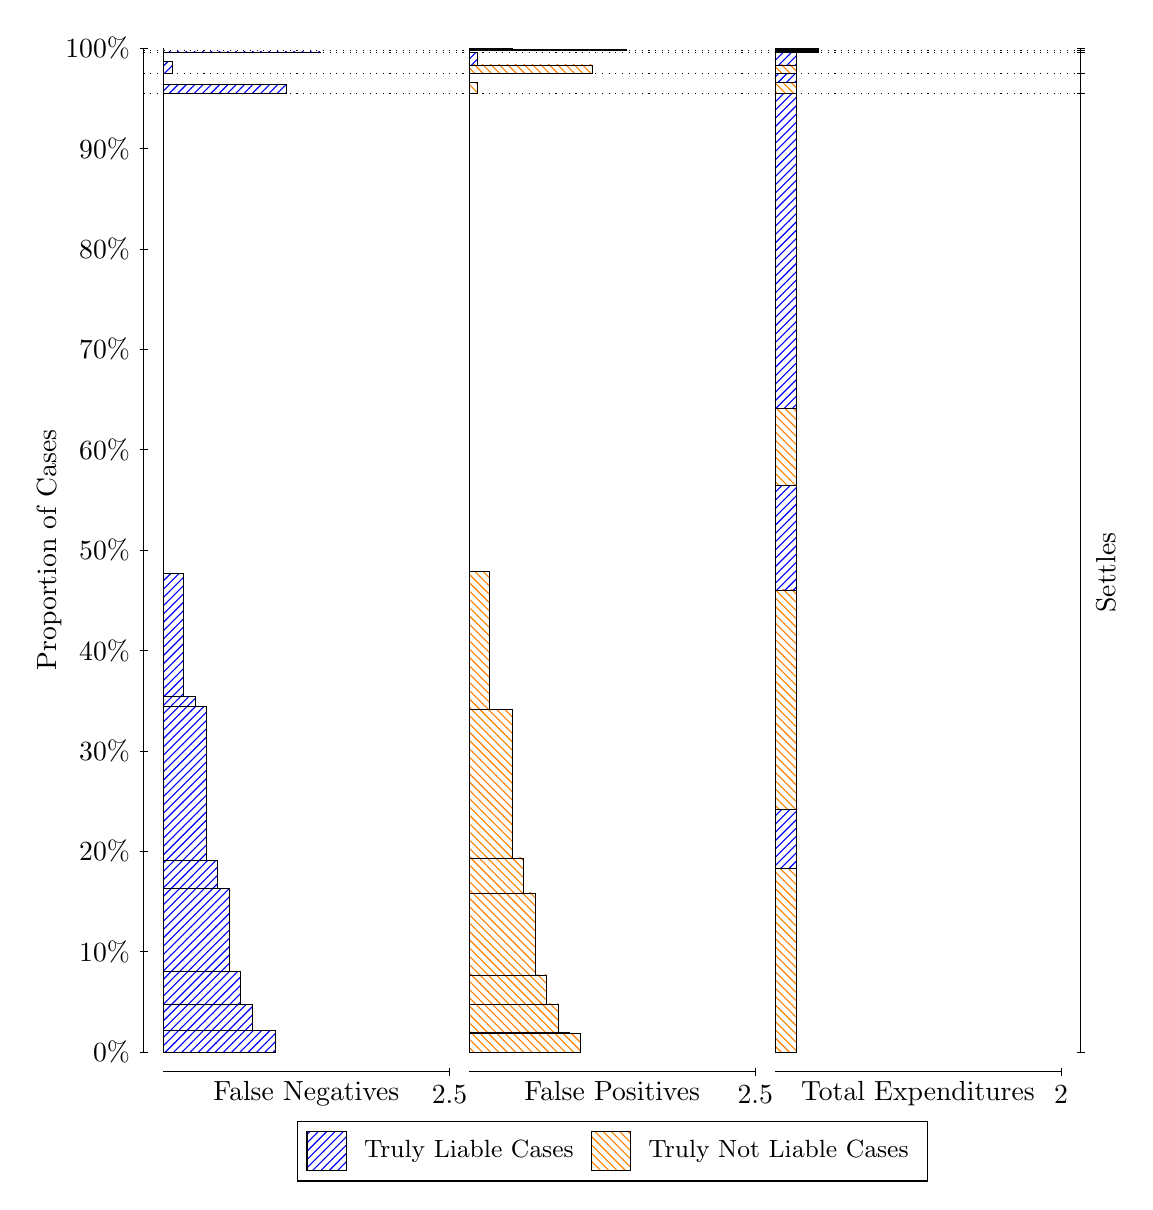
\begin{tikzpicture}
\draw[black, very thin] (1.5,1.75) -- (1.5,14.5);
\node[rotate=90, text=black, anchor=center] at (0.3, 8.125) {Proportion of Cases};
\draw[black, very thin] (1.45,1.75) -- (1.55,1.75);
\node[text=black, anchor=east] at (1.45, 1.75) {0\%};
\draw[black, very thin] (1.45,3.025) -- (1.55,3.025);
\node[text=black, anchor=east] at (1.45, 3.025) {10\%};
\draw[black, very thin] (1.45,4.3) -- (1.55,4.3);
\node[text=black, anchor=east] at (1.45, 4.3) {20\%};
\draw[black, very thin] (1.45,5.575) -- (1.55,5.575);
\node[text=black, anchor=east] at (1.45, 5.575) {30\%};
\draw[black, very thin] (1.45,6.85) -- (1.55,6.85);
\node[text=black, anchor=east] at (1.45, 6.85) {40\%};
\draw[black, very thin] (1.45,8.125) -- (1.55,8.125);
\node[text=black, anchor=east] at (1.45, 8.125) {50\%};
\draw[black, very thin] (1.45,9.4) -- (1.55,9.4);
\node[text=black, anchor=east] at (1.45, 9.4) {60\%};
\draw[black, very thin] (1.45,10.675) -- (1.55,10.675);
\node[text=black, anchor=east] at (1.45, 10.675) {70\%};
\draw[black, very thin] (1.45,11.95) -- (1.55,11.95);
\node[text=black, anchor=east] at (1.45, 11.95) {80\%};
\draw[black, very thin] (1.45,13.225) -- (1.55,13.225);
\node[text=black, anchor=east] at (1.45, 13.225) {90\%};
\draw[black, very thin] (1.45,14.5) -- (1.55,14.5);
\node[text=black, anchor=east] at (1.45, 14.5) {100\%};

\draw[black, very thin] (13.4,1.75) -- (13.4,14.5);
\draw[black, very thin] (13.35,1.75) -- (13.45,1.75);
\node[anchor=west] at (13.35, 1.75) {};
\draw[black, very thin] (13.35,13.928) -- (13.45,13.928);
\node[anchor=west] at (13.35, 13.928) {};
\draw[black, very thin] (13.35,14.176) -- (13.45,14.176);
\node[anchor=west] at (13.35, 14.176) {};
\draw[black, very thin] (13.35,14.443) -- (13.45,14.443);
\node[anchor=west] at (13.35, 14.443) {};
\draw[black, very thin] (13.35,14.471) -- (13.45,14.471);
\node[anchor=west] at (13.35, 14.471) {};
\draw[black, very thin] (13.35,14.5) -- (13.45,14.5);
\node[anchor=west] at (13.35, 14.5) {};

\draw[black, very thin, pattern color=blue, pattern=north east lines] (1.75,1.75) rectangle (3.167,2.0237);
\draw[black, very thin, pattern color=blue, pattern=north east lines] (1.75,2.0237) rectangle (2.8763,2.3564);
\draw[black, very thin, pattern color=blue, pattern=north east lines] (1.75,2.3564) rectangle (2.731,2.7745);
\draw[black, very thin, pattern color=blue, pattern=north east lines] (1.75,2.7745) rectangle (2.5857,3.8256);
\draw[black, very thin, pattern color=blue, pattern=north east lines] (1.75,3.8256) rectangle (2.4403,4.1831);
\draw[black, very thin, pattern color=blue, pattern=north east lines] (1.75,4.1831) rectangle (2.295,6.1416);
\draw[black, very thin, pattern color=blue, pattern=north east lines] (1.75,6.1416) rectangle (2.1497,6.2674);
\draw[black, very thin, pattern color=blue, pattern=north east lines] (1.75,6.2674) rectangle (2.0043,7.8294);
\draw[black, very thin, pattern color=orange, pattern=north west lines] (1.75,7.8294) rectangle (1.75,13.928);
\draw[black, very thin, pattern color=blue, pattern=north east lines] (1.75,13.928) rectangle (3.3123,14.036);
\draw[black, very thin, pattern color=orange, pattern=north west lines] (1.75,14.036) rectangle (1.75,14.176);
\draw[black, very thin, pattern color=blue, pattern=north east lines] (1.75,14.176) rectangle (1.859,14.333);
\draw[black, very thin, pattern color=orange, pattern=north west lines] (1.75,14.333) rectangle (1.75,14.443);
\draw[black, very thin, pattern color=blue, pattern=north east lines] (1.75,14.443) rectangle (3.7483,14.452);
\draw[black, very thin, pattern color=orange, pattern=north west lines] (1.75,14.452) rectangle (1.75,14.471);
\draw[black, very thin, pattern color=orange, pattern=north west lines] (1.75,14.471) rectangle (1.75,14.48);
\draw[black, very thin, pattern color=blue, pattern=north east lines] (1.75,14.48) rectangle (1.75,14.5);
\draw[black, very thin, pattern color=orange, pattern=north west lines] (5.6333,1.75) rectangle (7.0503,1.9832);
\draw[black, very thin, pattern color=orange, pattern=north west lines] (5.6333,1.9832) rectangle (6.905,2.0031);
\draw[black, very thin, pattern color=orange, pattern=north west lines] (5.6333,2.0031) rectangle (6.7597,2.3615);
\draw[black, very thin, pattern color=orange, pattern=north west lines] (5.6333,2.3615) rectangle (6.6143,2.7303);
\draw[black, very thin, pattern color=orange, pattern=north west lines] (5.6333,2.7303) rectangle (6.469,3.7696);
\draw[black, very thin, pattern color=orange, pattern=north west lines] (5.6333,3.7696) rectangle (6.3237,4.2145);
\draw[black, very thin, pattern color=orange, pattern=north west lines] (5.6333,4.2145) rectangle (6.1783,6.102);
\draw[black, very thin, pattern color=orange, pattern=north west lines] (5.6333,6.102) rectangle (5.8877,7.8485);
\draw[black, very thin, pattern color=blue, pattern=north east lines] (5.6333,7.8485) rectangle (5.6333,13.928);
\draw[black, very thin, pattern color=orange, pattern=north west lines] (5.6333,13.928) rectangle (5.7423,14.067);
\draw[black, very thin, pattern color=blue, pattern=north east lines] (5.6333,14.067) rectangle (5.6333,14.176);
\draw[black, very thin, pattern color=orange, pattern=north west lines] (5.6333,14.176) rectangle (7.1957,14.285);
\draw[black, very thin, pattern color=blue, pattern=north east lines] (5.6333,14.285) rectangle (5.7423,14.443);
\draw[black, very thin, pattern color=orange, pattern=north west lines] (5.6333,14.443) rectangle (5.6333,14.462);
\draw[black, very thin, pattern color=blue, pattern=north east lines] (5.6333,14.462) rectangle (5.6333,14.471);
\draw[black, very thin, pattern color=orange, pattern=north west lines] (5.6333,14.471) rectangle (7.6317,14.48);
\draw[black, very thin, pattern color=blue, pattern=north east lines] (5.6333,14.48) rectangle (6.1783,14.5);
\draw[black, very thin, pattern color=orange, pattern=north west lines] (9.5167,1.75) rectangle (9.7892,4.0824);
\draw[black, very thin, pattern color=blue, pattern=north east lines] (9.5167,4.0824) rectangle (9.7892,4.8332);
\draw[black, very thin, pattern color=orange, pattern=north west lines] (9.5167,4.8332) rectangle (9.7892,7.619);
\draw[black, very thin, pattern color=blue, pattern=north east lines] (9.5167,7.619) rectangle (9.7892,8.9437);
\draw[black, very thin, pattern color=orange, pattern=north west lines] (9.5167,8.9437) rectangle (9.7892,9.9241);
\draw[black, very thin, pattern color=blue, pattern=north east lines] (9.5167,9.9241) rectangle (9.7892,13.928);
\draw[black, very thin, pattern color=orange, pattern=north west lines] (9.5167,13.928) rectangle (9.7892,14.067);
\draw[black, very thin, pattern color=blue, pattern=north east lines] (9.5167,14.067) rectangle (9.7892,14.176);
\draw[black, very thin, pattern color=orange, pattern=north west lines] (9.5167,14.176) rectangle (9.7892,14.285);
\draw[black, very thin, pattern color=blue, pattern=north east lines] (9.5167,14.285) rectangle (9.7892,14.443);
\draw[black, very thin, pattern color=orange, pattern=north west lines] (9.5167,14.443) rectangle (10.062,14.462);
\draw[black, very thin, pattern color=blue, pattern=north east lines] (9.5167,14.462) rectangle (10.062,14.471);
\draw[black, very thin, pattern color=orange, pattern=north west lines] (9.5167,14.471) rectangle (10.062,14.48);
\draw[black, very thin, pattern color=blue, pattern=north east lines] (9.5167,14.48) rectangle (10.062,14.5);
\draw[black, dotted] (1.5,13.928) -- (13.4,13.928);
\draw[black, dotted] (1.5,14.176) -- (13.4,14.176);
\draw[black, dotted] (1.5,14.443) -- (13.4,14.443);
\draw[black, dotted] (1.5,14.471) -- (13.4,14.471);
\draw[black, very thin] (1.75,1.5) -- (5.3833,1.5);
\node[text=black, anchor=north] at (3.5667, 1.5) {False Negatives};
\draw[black, very thin] (5.3833,1.45) -- (5.3833,1.55);
\node[text=black, anchor=north] at (5.3833, 1.45) {2.5};

\draw[black, very thin] (5.6333,1.5) -- (9.2667,1.5);
\node[text=black, anchor=north] at (7.45, 1.5) {False Positives};
\draw[black, very thin] (9.2667,1.45) -- (9.2667,1.55);
\node[text=black, anchor=north] at (9.2667, 1.45) {2.5};

\draw[black, very thin] (9.5167,1.5) -- (13.15,1.5);
\node[text=black, anchor=north] at (11.333, 1.5) {Total Expenditures};
\draw[black, very thin] (13.15,1.45) -- (13.15,1.55);
\node[text=black, anchor=north] at (13.15, 1.45) {2};

\node[text=black, centered, rotate=90] at (13.72, 7.839) {Settles};





\draw (7.449999999999999,1.5) node[draw=none] (baseCoordinate) {};
\begin{scope}[align=center]
        \matrix[scale=0.5, draw=black, below=0.5cm of baseCoordinate, nodes={draw}, column sep=0.1cm]{
            \node[rectangle, draw, minimum width=0.5cm, minimum height=0.5cm, pattern color=blue, pattern=north east lines] {}; &
            \node[draw=none, font=\small, text=black] (B) {Truly Liable Cases}; &
            \node[rectangle, draw, minimum width=0.5cm, minimum height=0.5cm, pattern color=orange, pattern=north west lines] {}; &
            \node[draw=none, font=\small, text=black] (B) {Truly Not Liable Cases}; \\
            };
\end{scope}

\end{tikzpicture}
\end{document}